%%
%% Copyright 2019-2024 Elsevier Ltd
%%
%% Felex manuscript — Single-column CAS layout (primary submission version)
%% Target journal: Livestock Science (Elsevier)
%% Compile: pdflatex → bibtex → pdflatex × 2
%%

\documentclass[a4paper,fleqn]{cas-sc}

\usepackage[authoryear,longnamesfirst]{natbib}
\usepackage{algorithm}
\usepackage{algpseudocode}
\usepackage{lineno}

\begin{document}
\let\WriteBookmarks\relax
\def\floatpagepagefraction{1}
\def\textpagefraction{.001}
\linenumbers

% Short title (for running head)
\shorttitle{Felex: local livestock ration platform}

% Short author list (for running head)
\shortauthors{D.D. Kotelnikov and O.V. Demkina}

% Main title of the paper
\title[mode=title]{Felex: a local livestock ration decision-support platform for Russian small farms and animal businesses}

% Title footnote
\tnotemark[1]
\tnotetext[1]{This manuscript was submitted for publication in Livestock Science (Elsevier).}

% First author - Danil D. Kotelnikov
\author[1]{Danil D. Kotelnikov}[orcid=0009-0003-5159-5796]
\ead{danil.kotelnikov.02@mail.ru}
\ead[url]{https://github.com/danilkotelnikov/Felex}
\credit{Methodology, Software, Data curation, Formal analysis, Investigation, Writing - review \& editing, Visualization, Validation, Resources, Supervision, Project administration}
\affiliation[1]{organization={Far Eastern State Agrarian University},
                addressline={86 Politekhnicheskaya Str.},
                city={Blagoveshchensk},
                postcode={675005},
                state={Amur Oblast},
                country={Russia}}

% Second author - Olga V. Demkina (Corresponding)
\author[1]{Olga V. Demkina}[orcid=0000-0001-9303-4100]
\cormark[1]
\ead{demkina1976@gmail.com}
\credit{Conceptualization, Writing - original draft preparation}

% Corresponding author text
\cortext[cor1]{Corresponding author}

% Abstract (structured per Livestock Science requirements)
\begin{abstract}
\textbf{Background and objectives:} Mathematical ration formulation remains a core decision-support task in livestock production. For Russian small farms and animal businesses, software choice is constrained by regional feed data, mixed normative practice, intermittent connectivity, and limited tolerance for opaque cloud dependence. Felex was developed as a hybrid desktop application (Rust--React--Tauri) that implements transparent linear-programming workflows for ration calculation together with a local agent layer for bounded result interpretation.

\textbf{Data collection:} The raw normalized feed export contained 2,723 records. The benchmark-ready catalog contained 1,342 priced feed items assembled from 151 direct price anchors and 1,191 inferred benchmark prices.

\textbf{Research methods:} The optimization benchmark executed 23 livestock scenarios across three workflows (\texttt{build\_from\_library}, \texttt{complete\_from\_library}, \texttt{selected\_only}), yielding 69 total runs. Two Qwen 3.5 configurations (4B/4096 and 9B/2048) were tested as bounded consultants on 12 tasks with web search disabled; benchmark telemetry recorded effective model/context and fallback status.

\textbf{Results:} Across all optimization runs, mean runtime was 246.6~ms, mean hard-constraint pass rate was 64.8\%, and mean norm coverage index was 81.8/100. The \texttt{complete\_from\_library} workflow achieved the highest coverage (85.0), while \texttt{selected\_only} was fastest (0.41~ms). Both agent configurations scored identically (overall applicability 34.2/100) with no hidden fallback.

\textbf{Conclusions:} Felex demonstrates that a locally deployable livestock ration platform can combine transparent optimization, mixed normative support, and a practical desktop runtime without relying on cloud-first architecture.

\textbf{Contributions:} Main strengths are local deployment and explicit workflows; current limits are database coverage, linear-model assumptions, and insufficient agent reliability for dependable consultation.
\end{abstract}

% Graphical abstract omitted in this source build because no repository-backed
% graphical-abstract asset is currently present in the audited submission bundle.

% Research highlights (3-5 bullets, max 85 characters each per Elsevier)
\begin{highlights}
\item Local ration decision-support system for Russian small farms
\item Three optimization workflows benchmarked across 23 livestock scenarios
\item Expert-defined ration skeletons improved mean norm coverage to 85.0
\item Mean optimization runtime was 246.6 ms across all workflows
\item Local language model agents were inadequate for dependable consultation
\end{highlights}

% Keywords (1-7 terms, separated by \sep)
\begin{keywords}
livestock feeding \sep ration formulation \sep decision support \sep linear programming \sep desktop software \sep Russia
\end{keywords}

\maketitle

% Main text
\section{Introduction}\label{sec:introduction}

Mathematical ration formulation remains a core decision-support task in livestock production because biological requirements, feed availability, and ration cost must be balanced simultaneously \citep{nASEM2021, dantzig1963, zhai2020, tedeschi2021smart}. In practice, software for this task already spans enterprise formulation suites, consultant-oriented desktop tools, and farm-management platforms \citep{datacor2026, mixit2026, winfeed2026, korall2026, deltakorm2026, onecow2026, winmix2026}. The field is therefore not empty; the practical problem is heterogeneity. US/EN products show stronger commercial and enterprise maturity, whereas Russian products are more localized to domestic workflows but are predominantly closed and vendor-specific.

For Russian small farms and animal businesses, software choice is additionally constrained by regional feed data, mixed normative practice, intermittent connectivity, and limited tolerance for opaque cloud dependence \citep{kalashnikov2003, vizh2020, aquilani2022, selvaggi2024}. In this setting, a useful instrument does not need to replace enterprise suites. It needs to provide transparent local optimization, practical norm handling, and reproducible workflow support while remaining usable by specialists outside large integrated software stacks.

Felex was developed in response to that narrower use case. It is a hybrid desktop application (Rust--React--Tauri) that implements linear programming workflows for ration calculation and includes a local agent layer for result interpretation. The objective of this paper is to describe the current executable architecture, report benchmarked optimizer performance, and assess whether the present local-agent layer is suitable for supportive interpretation of calculated rations in a practical livestock workflow.

\section{Materials and Methods}\label{sec:methods}

\subsection{System architecture}\label{subsec:architecture}

Felex utilizes a multi-tiered modular architecture separating the user interface, optimization runtime, and data layer. The frontend is implemented in React 18 and TypeScript with Zustand-based state management. The optimization backend is written in Rust \citep{rust2023} and uses \texttt{good\_lp} \citep{goodlp2023} for linear programming. Desktop packaging is provided by Tauri \citep{tauri2023}, but the runtime is not pure Tauri IPC: the desktop shell launches an embedded local HTTP backend, and the frontend communicates with the optimizer through the same API surface used in local-browser development. The local data layer relies on SQLite supplemented by generated JSON artifacts.

The agent layer defaults to Ollama in the current repository configuration but also supports OpenAI-compatible endpoints. In the present benchmark, the agent was treated as a bounded consultant rather than as an autonomous formulation module, and all agent tests were executed with web search disabled.

The executable interaction among these components is summarized in Figure~\ref{fig:architecture}.

\begin{figure}[htbp]
    \centering
    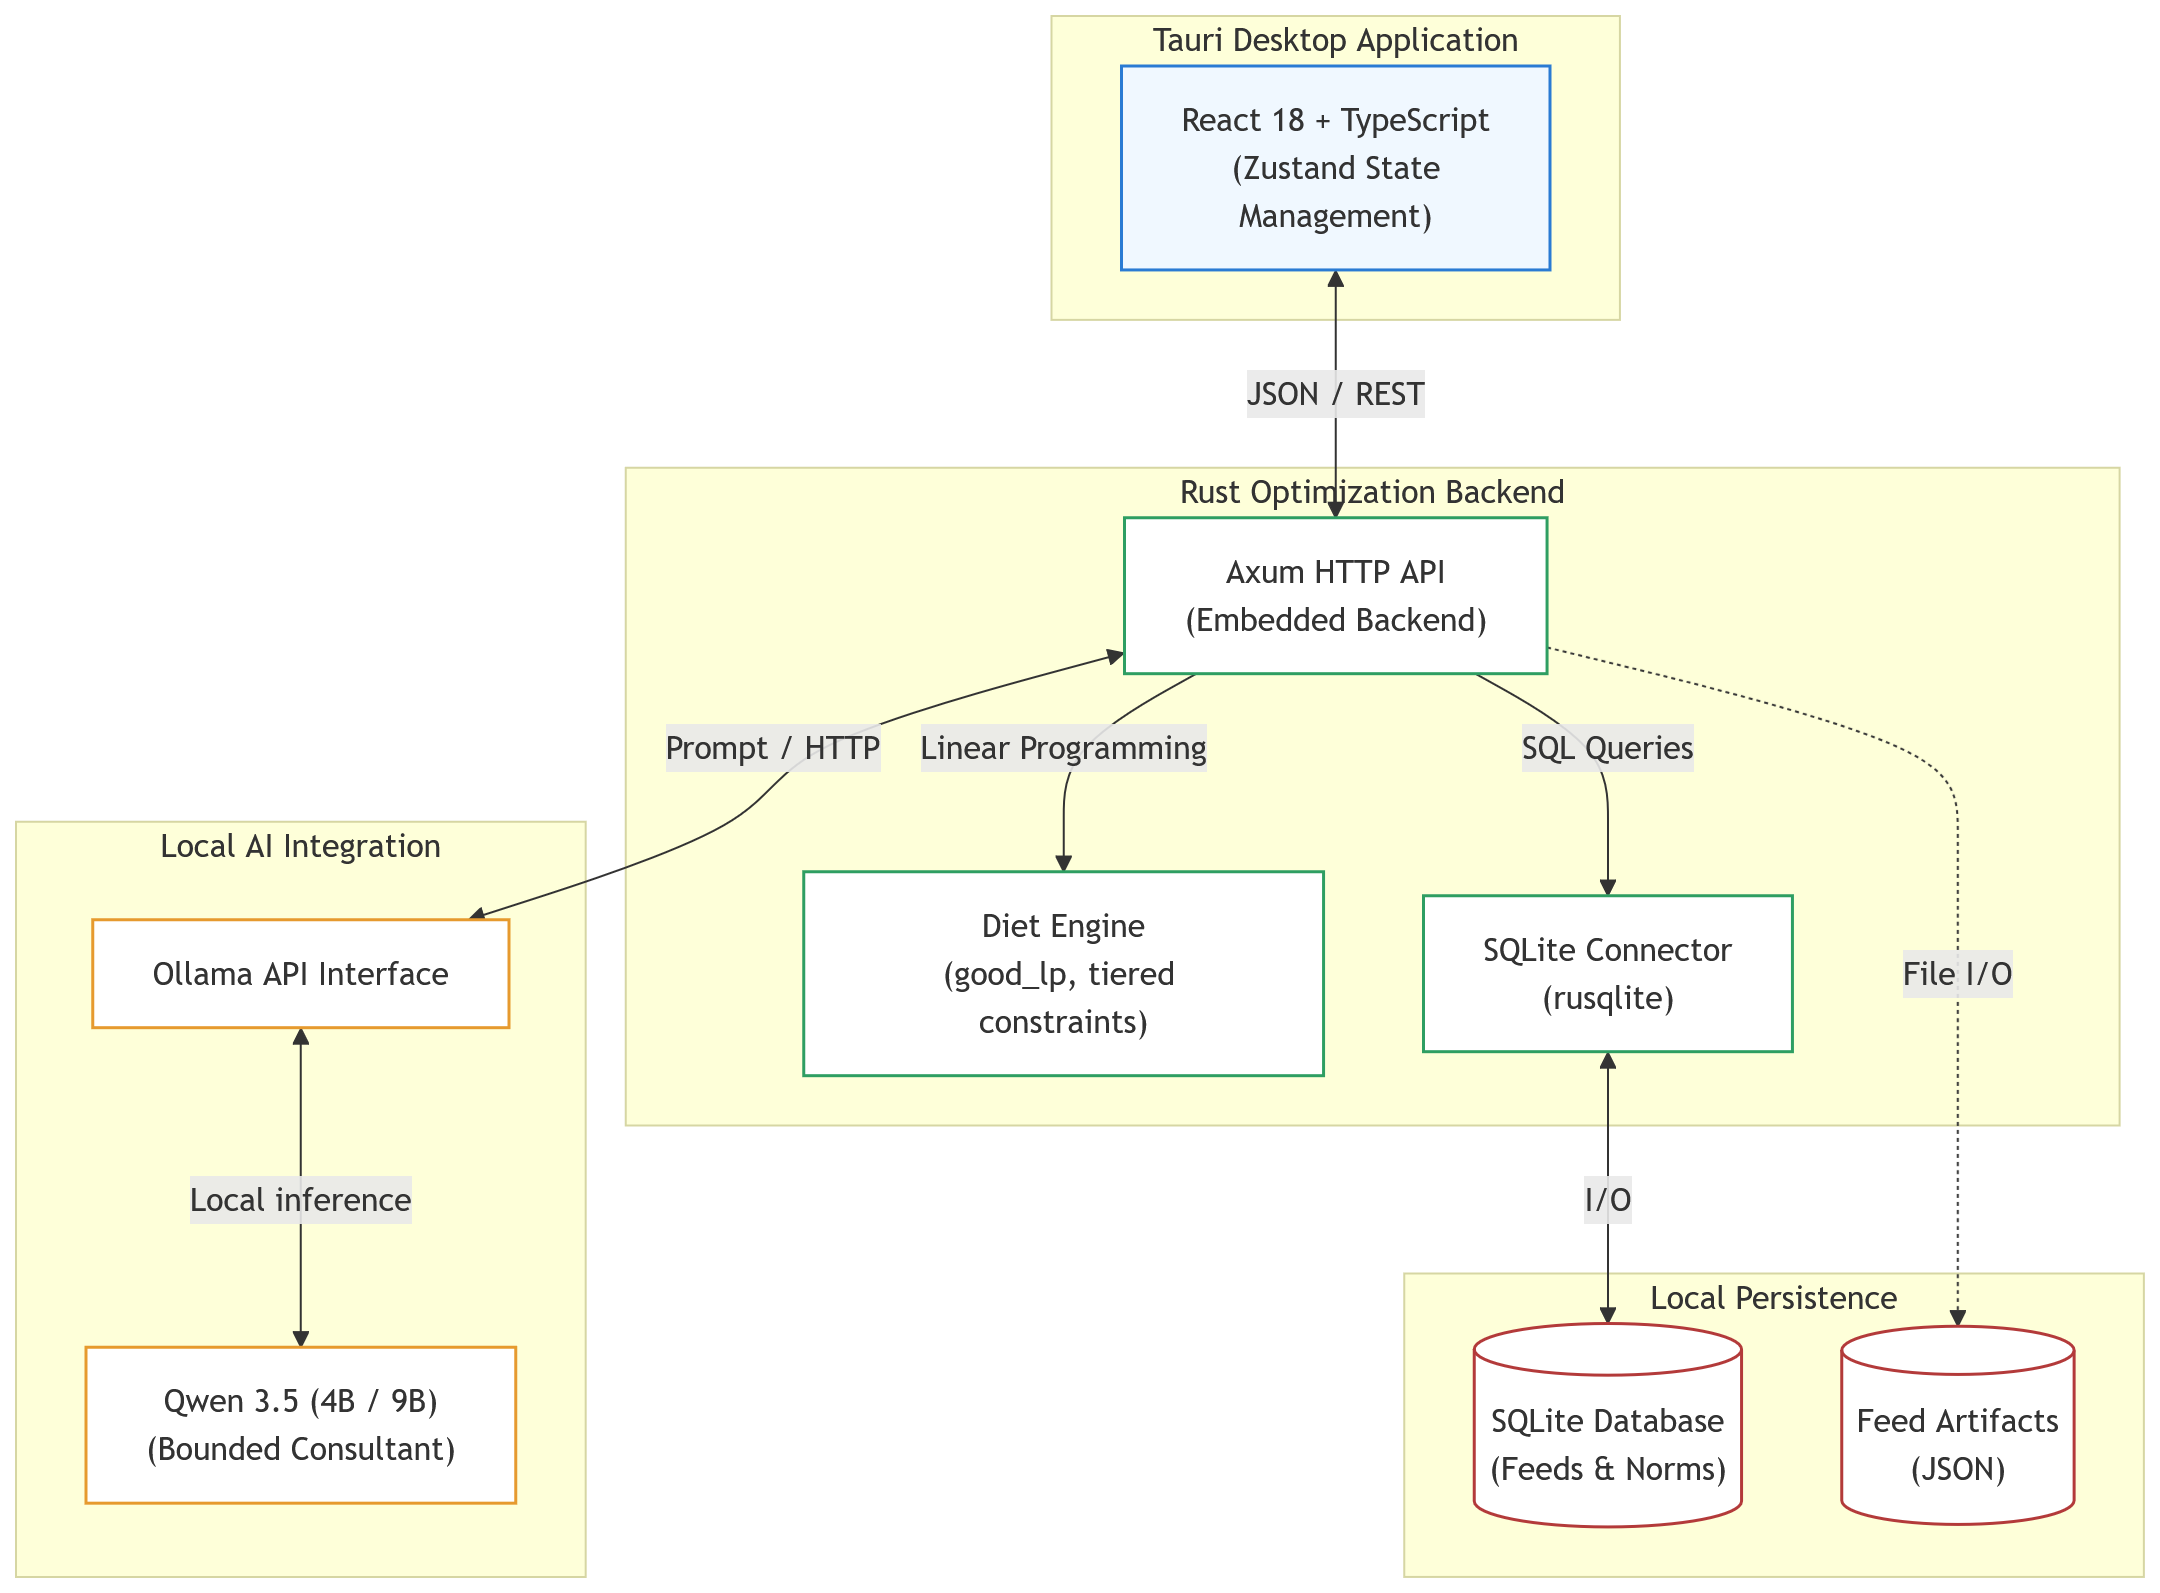
\includegraphics[width=0.95\textwidth]{Figure_1_System_Architecture.png}
    \caption{Felex system architecture, illustrating the interaction between the React user interface, the embedded Rust HTTP backend, the local database, and the local agent layer.}
    \label{fig:architecture}
\end{figure}

\subsection{Feed database and nutrient system}\label{subsec:database}

The foundation of the algorithm is a feed database obtained through automated extraction and systematization of information from the open directory vidkormov.narod.ru. A custom Python pipeline handles data collection, translation, and normalization, compiling a local SQLite database. The raw normalized export currently contains 2,723 feed records. The benchmark-ready priced catalog used in the present publication artifact contains 1,342 feed items, assembled from 151 direct price anchors and 1,191 benchmark-priced records after fallback matching. The library spans roughage, succulents, concentrates, protein supplements, minerals, premixes, industrial by-products, animal-origin feeds, and non-protein nitrogen (NPN) sources.

\textbf{Prices in the benchmark catalog are synthetic and used for workflow evaluation purposes only}; they do not represent real-time market data. The raw normalized export (2,723 records) serves as reference data without price information.

The embedded database schema (\texttt{feeds}) supports a core contour of 31 nutrient and related feed-composition fields used by the ration engine. These include dry matter, three species-specific metabolizable energy indicators (\texttt{energy\_oe\_cattle}, \texttt{energy\_oe\_pig}, \texttt{energy\_oe\_poultry}), crude and digestible protein (\texttt{dig\_protein\_cattle}, \texttt{dig\_protein\_pig}, \texttt{dig\_protein\_poultry}), amino acids (lysine, methionine + cystine), crude fat, crude fiber, starch, sugar, macro- and microelements (Ca, P, Mg, K, Na, S, Fe, Cu, Zn, Mn, Co, I), and vitamins/precursors (carotene, vitamins D3 and E). Derived ratios and percentage constraints are then formed inside the optimizer from these stored fields.

The use of species-specific energy metrics is dictated by fundamental differences in digestion. For ruminants (cattle), the energy value of feed is evaluated based on metabolizable energy (\texttt{energy\_oe\_cattle}) accounting for rumen fermentation processes, which conceptually aligns with modern nutritional evaluation models \citep{sauvant2018, nASEM2021}. For monogastric animals, the metrics \texttt{energy\_oe\_pig} and \texttt{energy\_oe\_poultry} are used. The units of measurement for norms also depend on the animal species: for cattle, absolute daily values (e.g., MJ and grams per day) are predominantly used, whereas for swine and poultry, relative concentrations (g/kg of feed or percentages of the ration) are applied.

An important feature of the system for monogastric animals is digestibility-aware handling of amino-acid constraints. The current implementation interprets standardized ileal digestibility (SID) and true ileal digestibility (TID) requirements through the norm and optimizer layer, with alias/fallback handling where fully separated feed-profile fields are unavailable. The transition from evaluating total amino acid content to ileal-digestible forms remains a global standard \citep{stein2007, nRC2012, nRC1994}, because it allows a more accurate assessment of biological protein availability and reduces excess nitrogen excretion \citep{pomar2021, deLange2012, vanmilgen2015}.

For benchmark cost evaluation, the engine first imports the latest non-inferred price anchors from the working Felex database and then fills the remaining benchmark catalog through an explicit fallback pipeline based on subcategory, category, family, and global medians. This produces a fully priced benchmark catalog while preserving provenance labels for direct versus inferred prices.

\subsection{Feeding norms and their derivation}\label{subsec:norms}

The system implements a multi-level process for calculating zootechnical norms: ranging from base values in database tables to species-specific dynamic models and factorial calculations. To ensure maximum accuracy, contextual scaling mechanisms are applied to the norms depending on the animal's physiological state (live weight, productivity, age, sex).

For lactating cows, a dynamic model is applied to estimate dry matter intake (DMI) and net energy for lactation (NEL). Energy requirements consist of maintenance metabolism, depending on metabolic body weight ($BW^{0.75}$), and lactation costs, calculated based on 4\% fat-corrected milk (FCM). Base equations and breed correction factors are adapted from classical methodologies \citep{nRC2001, kalashnikov2003}.

For finishing pigs, bilinear interpolation of normative tables by live weight and average daily gain is used. The model dynamically calculates requirements for metabolizable energy, protein, and standardized ileal-digestible amino acids, scaling them based on the expected growth intensity \citep{nRC2012}.

Poultry nutrition accounting considers phase feeding. For broilers, amino acid requirements (TID lysine, TID methionine+cystine) are specified as strict percentages of the ration depending on the rearing period (starter, grower, finisher) \citep{vnitip2017, nRC1994}. For laying hens, a factorial approach is used to calculate calcium, summing maintenance requirements for life and shell formation costs depending on egg production.

The computational core is based on a software factorial framework (\texttt{NutrientCalculator}), which sums requirement components (maintenance, growth, production, lactation, gestation) considering absorption coefficients. The differences in the units of measurement used for norms are fundamental: ruminants consume large volumes of roughage with variable composition, so the balance is maintained in absolute daily amounts per head, whereas monogastric animals receive complete compounded feeds with strictly controlled nutrient concentrations (percentages or g/kg).

\subsection{Feed structural matrix}\label{subsec:matrix}

To ensure the biological adequacy of the ration, in addition to nutrient balance, it is necessary to adhere to structural proportions. For this purpose, a feed matrix is integrated into the optimizer, specifying allowable boundaries (minimum, optimum, maximum as a percentage of dry matter) for various feed categories.

The system automatically classifies each ingredient (\texttt{classify\_feed}), assigning it to one of the functional groups: roughage, concentrate, succulent, mineral, premixes, animal-origin feeds, or non-protein nitrogen (NPN) sources. Based on these categories, species-specific structural constraints are imposed. For instance, to maintain normal rumen physiology in dairy cattle, the proportion of roughage must range from 35\% to 65\% of dry matter, while broiler rations consist almost entirely of concentrates.

An exception to strict matrix rules is made for certain physiological groups, such as gestating sows, whose ration is primarily formulated based on individual inclusion limits of specific ingredients and target caloric content. In addition to matrix proportions, the engine supports individual constraints on the maximum inclusion percentage for specific feeds (e.g., strict control over urea inclusion or high-fat feeds).

\subsection{Optimization core mathematical model and workflows}\label{subsec:optimization}

The Felex engine formulates the ration construction task as a linear programming problem with hierarchical constraints (tiered constraints). Let $x \in \mathbb{R}^n$ denote the vector of feed quantities used (in kg of natural or dry matter), where $n$ is the total number of available ingredients. The cost vector for the feeds is denoted as $c \in \mathbb{R}^n$. The objective function seeks to minimize the total cost of the ration:
\begin{equation}
\min_{x} \quad z = c^T x
\end{equation}

The model constraints are defined by the nutrient composition matrix $A \in \mathbb{R}^{m \times n}$ and the vectors of the animal's minimum $b_{\min} \in \mathbb{R}^m$ and maximum $b_{\max} \in \mathbb{R}^m$ requirements:
\begin{equation}
b_{\min} \leq A x \leq b_{\max}, \quad x \geq 0
\end{equation}

To ensure the problem remains solvable under conflicting requirements, an additive hierarchy of constraints is applied. Note that absolute limits (e.g., maximum dry matter intake, feed structural matrix) are applied as non-relaxable LP constraints outside the tier system. The nutrient constraints are divided into three tiers:
\begin{itemize}
    \item \textbf{Tier 1}: Essential (hard) nutrients (metabolizable energy, crude protein, calcium, phosphorus).
    \item \textbf{Tier 2}: Standard nutrients (lysine, methionine, crude fiber). The system supports fallback mechanisms: for instance, if standardized ileal digestible lysine (\texttt{lysine\_sid}) is missing from a feed profile, the general \texttt{lysine} value is used.
    \item \textbf{Tier 3}: Soft constraints, such as trace elements and vitamins (zinc, copper, vitamins E and D3).
\end{itemize}

The optimizer implements three conceptual workflows:
\begin{enumerate}
    \item \texttt{build\_from\_library}: Automatic construction (unbounded search). A structural feed matrix is applied to enforce acceptable category proportions (e.g., ``roughage $\geq 40\%$ DM'').
    \item \texttt{complete\_from\_library}: Balancing a user-defined ration ``skeleton''. The user's constraints on specific ingredients are fixed, and missing nutrients are covered from the library.
    \item \texttt{selected\_only}: Bounded search restricted exclusively to user-selected feeds, without the ability to introduce new ingredients.
\end{enumerate}

The optimizer's workflow (Algorithm \ref{alg:optimizer}) uses an additive constraint-building method, locking the achieved target levels from the previous tier. In case of infeasibility in the strict tiered problem, a goal programming mechanism (soft goals with penalty functions) is applied.

\begin{algorithm}[htbp]
\caption{Additive Hierarchical Ration Optimization Algorithm (Diet Engine)}\label{alg:optimizer}
\begin{algorithmic}[1]
\Require Cost vector $c$, nutrient matrix $A$, requirement vectors $b_{\min}, b_{\max}$, set of available feeds $F$.
\Ensure Optimal vector $x^*$.
\State $T \gets \emptyset$ \Comment{Current set of constraints (beyond base intake limits)}
\State $B \gets \emptyset$ \Comment{Locked target bands for previously achieved nutrients}
\For{$L \in \{\text{Tier 1}, \text{Tier 2}, \text{Tier 3}\}$}
    \State $T \gets T \cup L$
    \State Solve LP subproblem: optimize objective function for nutrients $T$ considering bands $B$.
    \If{Solution $x$ is found}
        \State Update $x^* \gets x$
        \State Add achieved nutrient levels from $L$ to bands $B$ (with tolerance).
    \Else
        \State \textbf{break}
    \EndIf
\EndFor
\If{$x^*$ is Null (infeasible even for Tier 1)}
    \State $x^* \gets \text{solution using goal programming (weighted penalties)}$.
\Else
    \State Perform final cost minimization: $\min c^T x$ subject to bands $B$.
\EndIf
\State \Return $x^*$ and the achieved nutrient profile $A x^*$.
\end{algorithmic}
\end{algorithm}

\subsection{Computational experiment methodology and artifact generation}\label{subsec:experiment}

To evaluate practical performance, computational testing was conducted using the canonical benchmark artifact generated by the current Felex benchmark pipeline. The authored scenario catalog contains 40 scenarios, but the executable benchmark currently runs 23 implemented livestock scenarios (dairy and beef cattle, swine, poultry; Supplementary Table S1). Scenario-level optimization outcomes for those cases are reported in Supplementary Table S2. The benchmark-ready catalog contained 1,342 priced feed items; 151 had direct price anchors and the remaining 1,191 benchmark-priced records were generated through the fallback pricing pipeline. For each executed scenario, optimization was run under three workflows: \texttt{build\_from\_library}, \texttt{complete\_from\_library}, and \texttt{selected\_only}, yielding 69 total runs. Results (runtime, constraint fulfillment proportions, costs, deficiency/excess components, and norm-coverage scores) were exported programmatically to JSON and then converted into derived CSV tables and figure assets.

All graphs, tables, and statistical summaries were programmatically generated from the benchmark JSON to eliminate manual data transcription errors. To assess the overall quality of the resulting ration, the benchmark used the implemented Felex adequacy score (reported here as the Norm Coverage Index, scale 0--100). For each evaluable constraint $k$ with actual value $a_k$, lower bound $L_k$, upper bound $U_k$, and target $T_k$, the benchmark computed:
\begin{equation}
 d^-_k = \max\left(0, \frac{L_k - a_k}{L_k}\right), \qquad
 d^+_k = \max\left(0, \frac{a_k - U_k}{U_k}\right), \qquad
 g_k = \frac{|a_k - T_k|}{|T_k|}
\end{equation}
The aggregate score was then defined as
\begin{equation}
\text{Coverage} = \frac{100}{1 + \bar{P}}
\end{equation}
where $\bar{P}$ is the tier-weighted mean of $d^-_k + d^+_k + 0.25 g_k$ across the controlled constraint set, using the implemented Felex priority weights (Tier 1 = 3, Tier 2 = 2, Tier 3 = 1). Quality Delta was computed as the difference in this score between the \texttt{complete\_from\_library} and \texttt{build\_from\_library} workflows.

The local agent layer was evaluated as a bounded consultation assistant through the Felex-native agent stack rather than through direct Ollama prompts. All agent tests were run sequentially with web search disabled to reduce uncontrolled latency and background work. Two local configurations were tested: Qwen 3.5 4B at 4096 context tokens and Qwen 3.5 9B at 2048 context tokens \citep{qwen2023, ollama2023}. The benchmark included six ration-diagnosis tasks based on sparse starter rations and six feed-lookup tasks tied to the benchmark catalog. Metrics included limiting-nutrient recall@3, recommendation overlap@3, grounded recommendation rate@3, lookup accuracy, and an overall applicability score defined as $100 \times (0.45 \times \text{recall} + 0.25 \times \text{groundedness} + 0.10 \times \text{overlap} + 0.20 \times \text{lookup accuracy})$. Benchmark telemetry also recorded the effective model, effective context window, and whether hidden fallback occurred during any task. This evaluation was designed to assess bounded supportive adequacy, not autonomous advisory readiness.

\section{Results}\label{sec:results}

\subsection{Computational performance}\label{subsec:performance}

Analysis of the 69 runs revealed clear structural differences in performance among the workflows (Figure \ref{fig:runtime}). The mean optimization time across all tests was 246.6~ms. The \texttt{build\_from\_library} workflow was computationally the most expensive, averaging 617.5~ms, because it searches the broadest ingredient space under matrix and norm constraints. The \texttt{complete\_from\_library} workflow averaged 121.8~ms, whereas the strictly bounded \texttt{selected\_only} workflow averaged only 0.41~ms. Workflow-level summary statistics are provided in Supplementary Table S3, while species-level benchmark aggregates used later for economic interpretation are summarized in Supplementary Table S4. Under the current benchmark, all three workflows therefore remain operationally interactive, with the main trade-off being search breadth rather than unacceptable latency.

\begin{figure}[htbp]
    \centering
    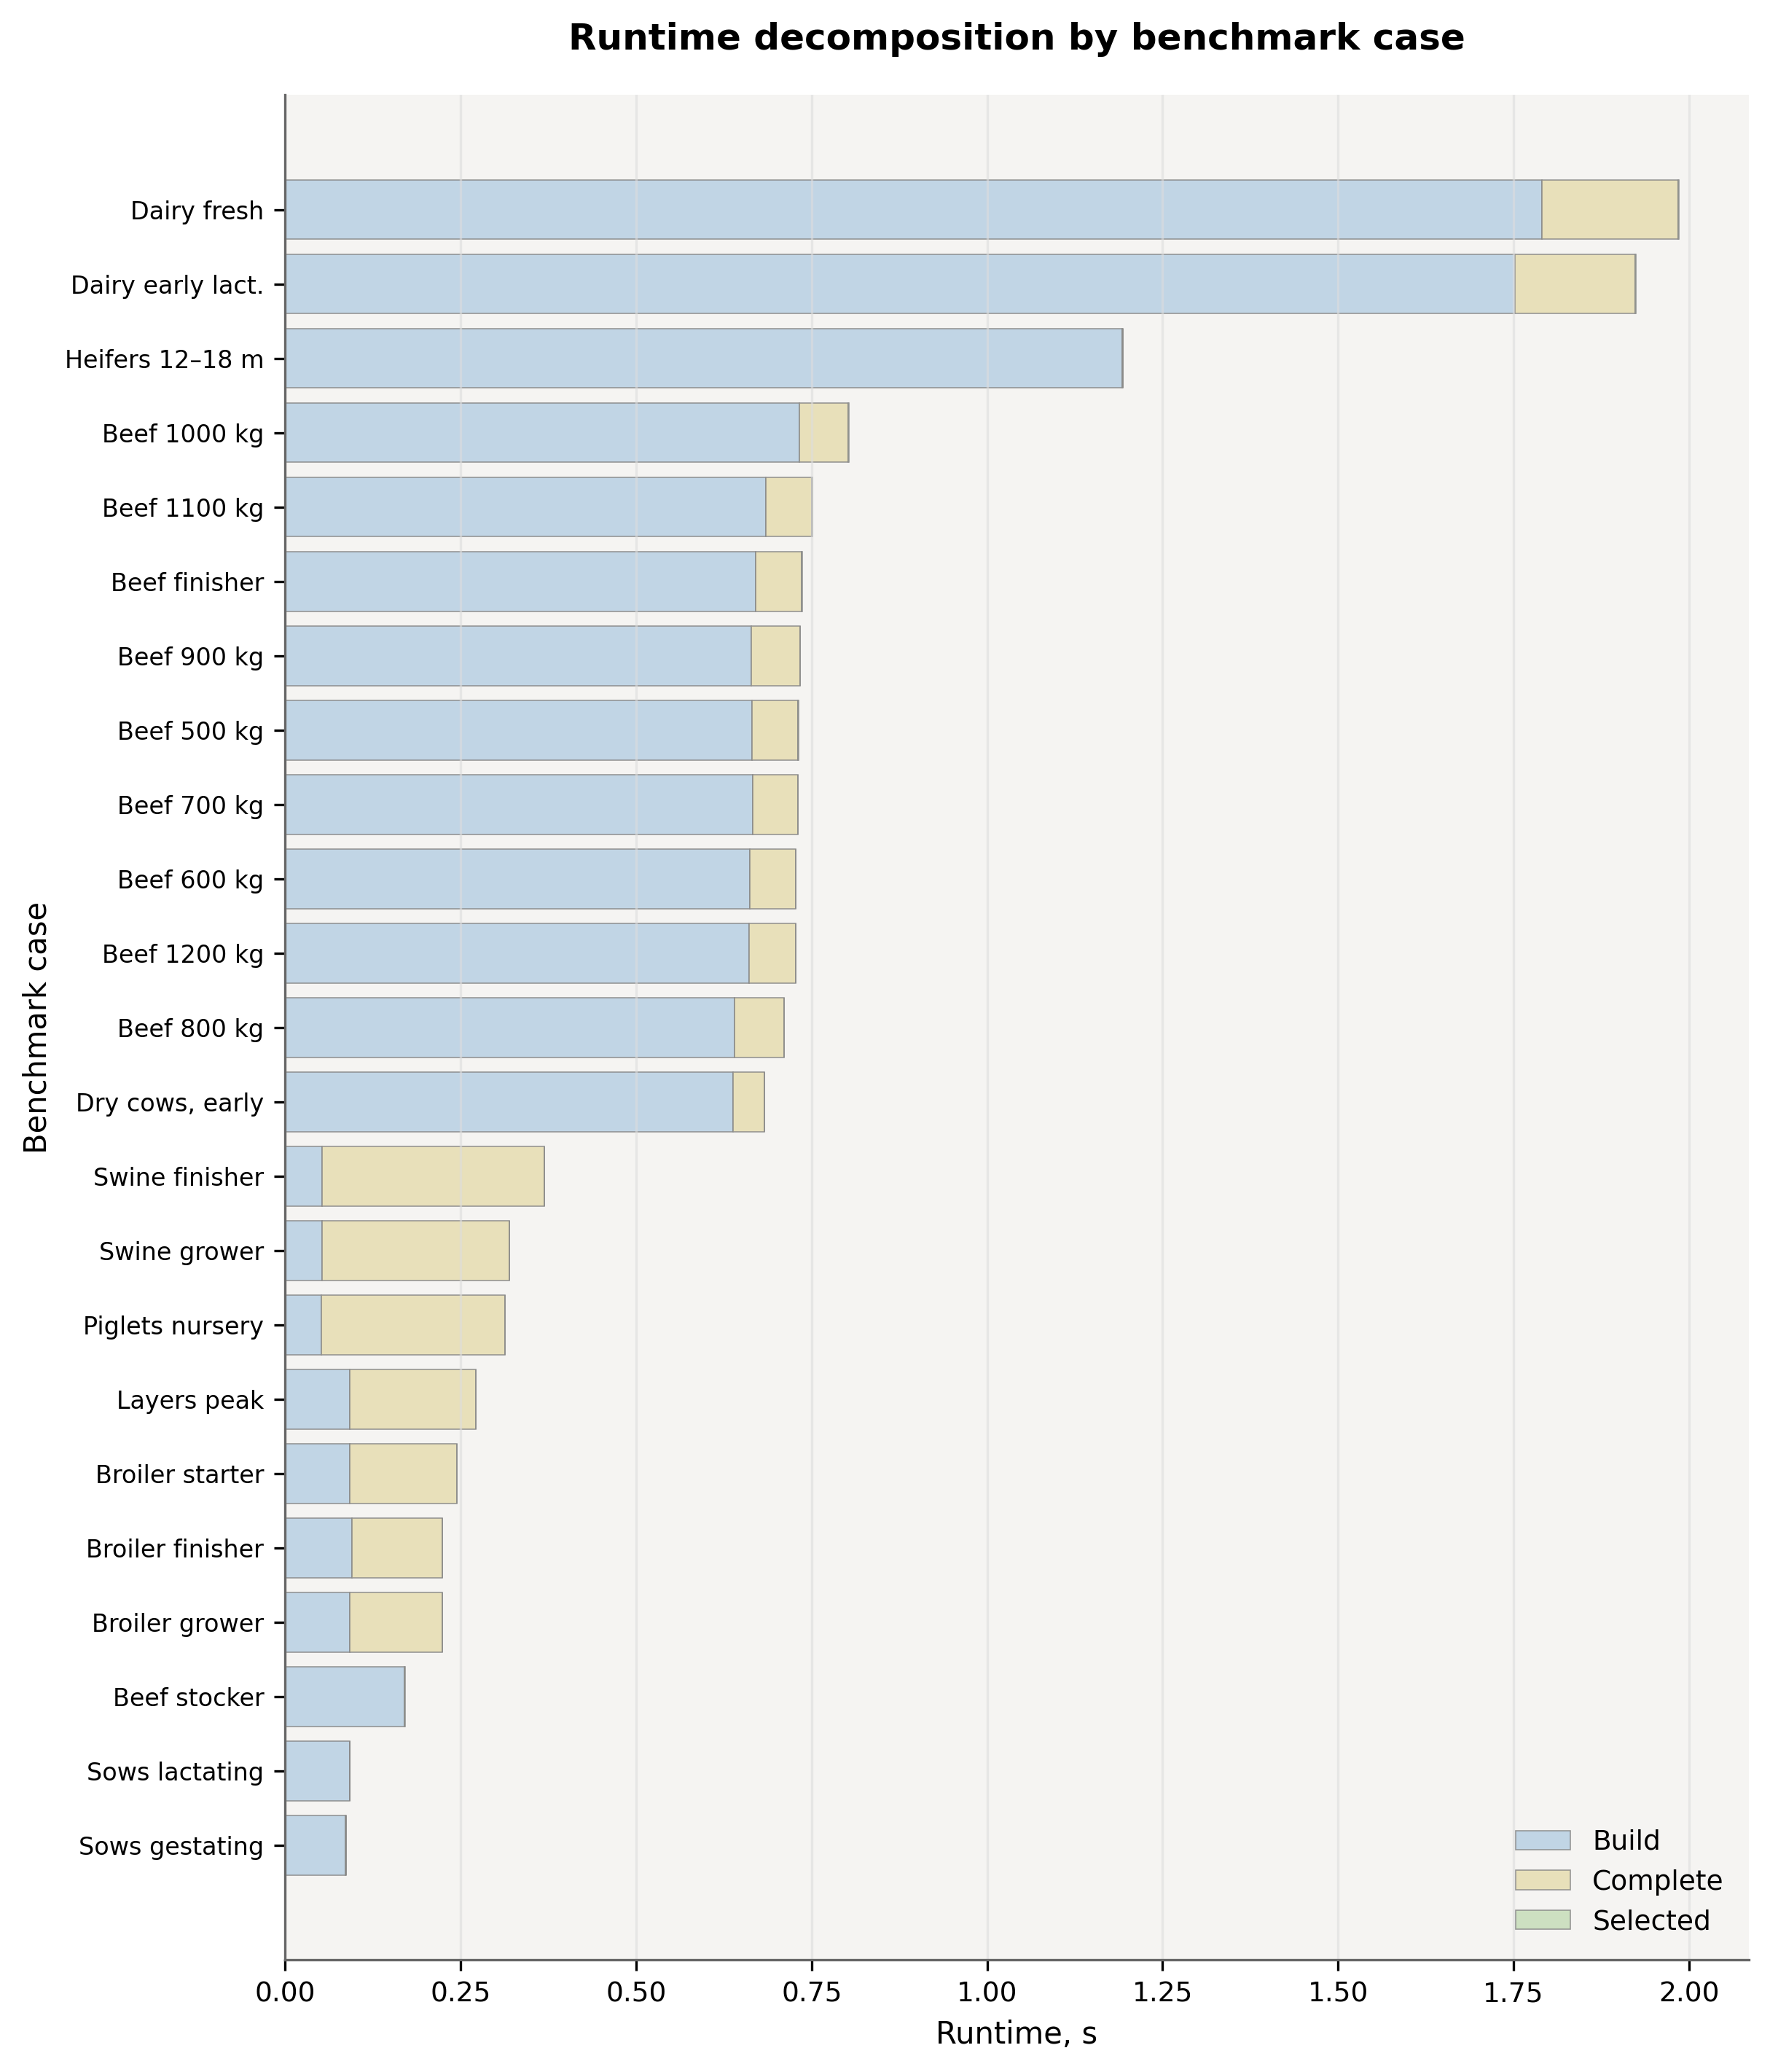
\includegraphics[width=0.88\textwidth]{Figure_4_Runtime.png}
    \caption{Comparison of execution times (Runtime) across workflows and scenarios. The bars demonstrate the relative contribution of each mode to the total computational time.}
    \label{fig:runtime}
\end{figure}

\subsection{Norm coverage quality and deficiency structure}\label{subsec:quality}

The mean pass rate for hard constraints was 64.8\%, and the average Norm Coverage Index across the entire sample was 81.8 out of 100.

The impact of preliminary manual intervention on ration quality is demonstrated in Figures \ref{fig:qualitypoints} and \ref{fig:qualitydelta}. The \texttt{complete\_from\_library} mode (coverage 85.0) systematically improved ration quality compared to automatic building from scratch (coverage 83.2), highlighting the value of an expert-defined ``skeleton'' (e.g., fixed roughage volumes). The Quality Delta was most pronounced in cattle scenarios. Conversely, the \texttt{selected\_only} mode exhibited the lowest coverage (77.1) due to the artificially narrowed ingredient list.

\begin{figure}[htbp]
    \centering
    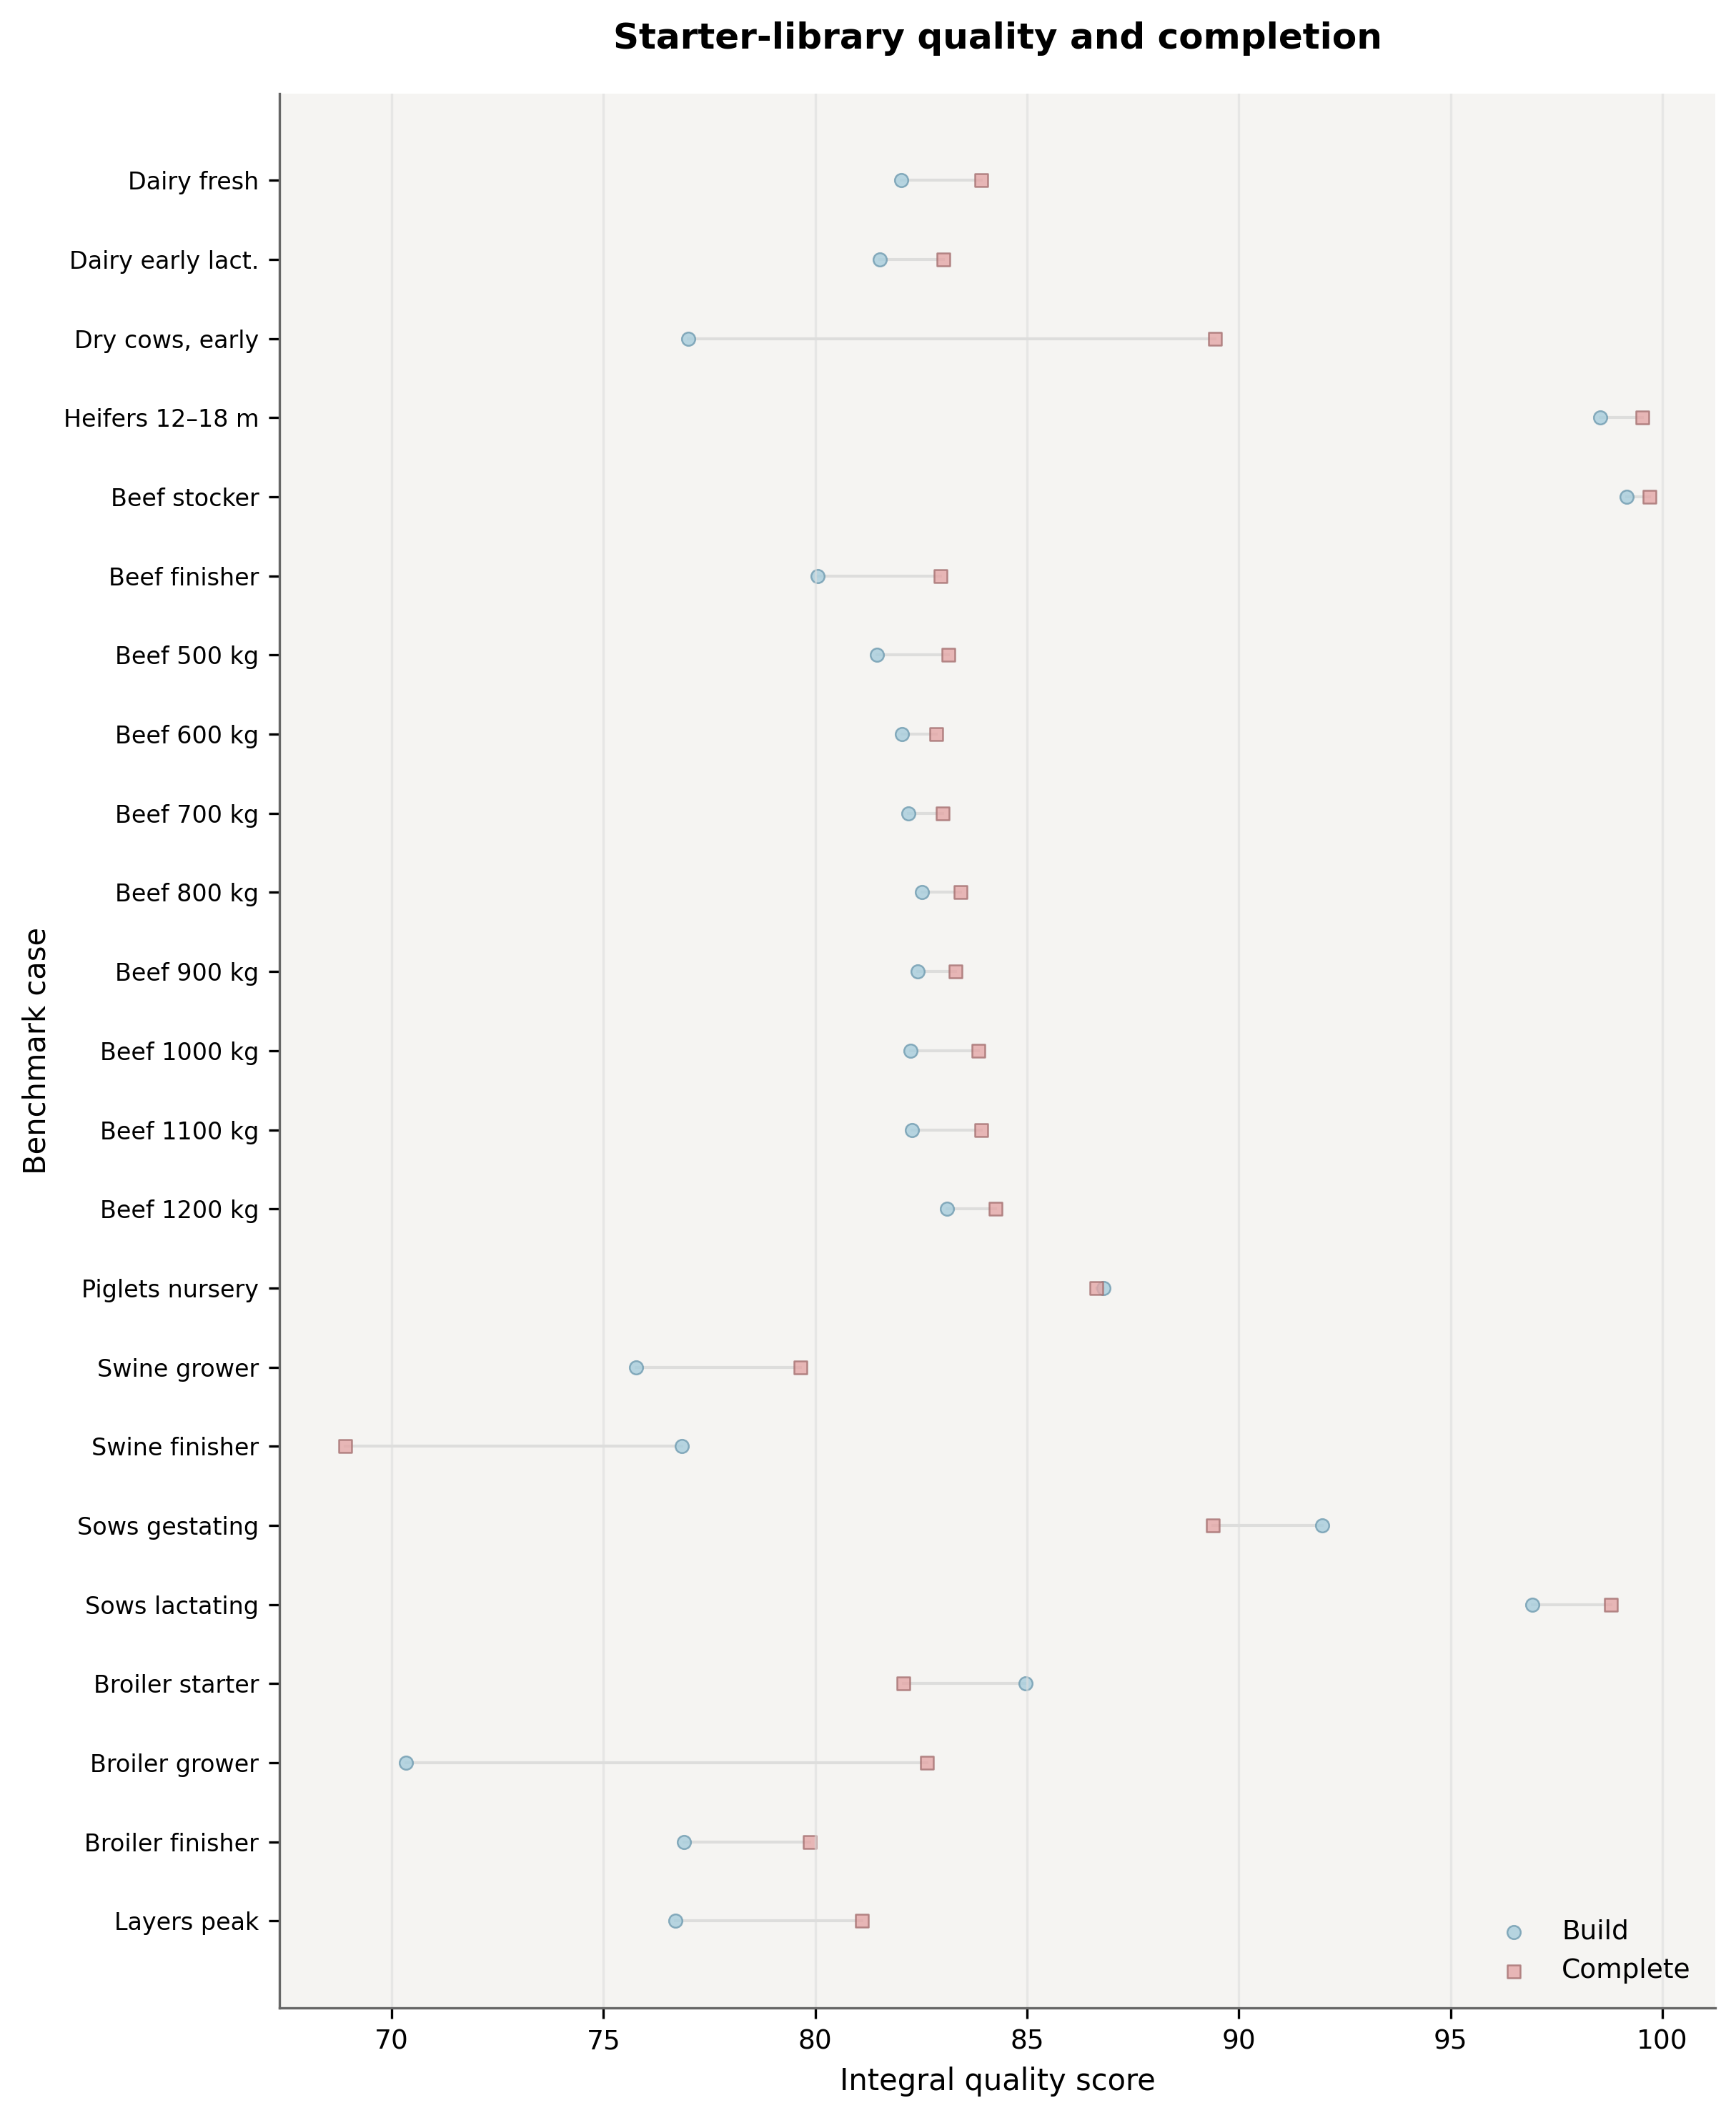
\includegraphics[width=0.85\textwidth]{Figure_2_Quality_Points.png}
    \caption{Comparison of the Norm Coverage index between the \texttt{build\_from\_library} and \texttt{complete\_from\_library} modes.}
    \label{fig:qualitypoints}
\end{figure}

\begin{figure}[htbp]
    \centering
    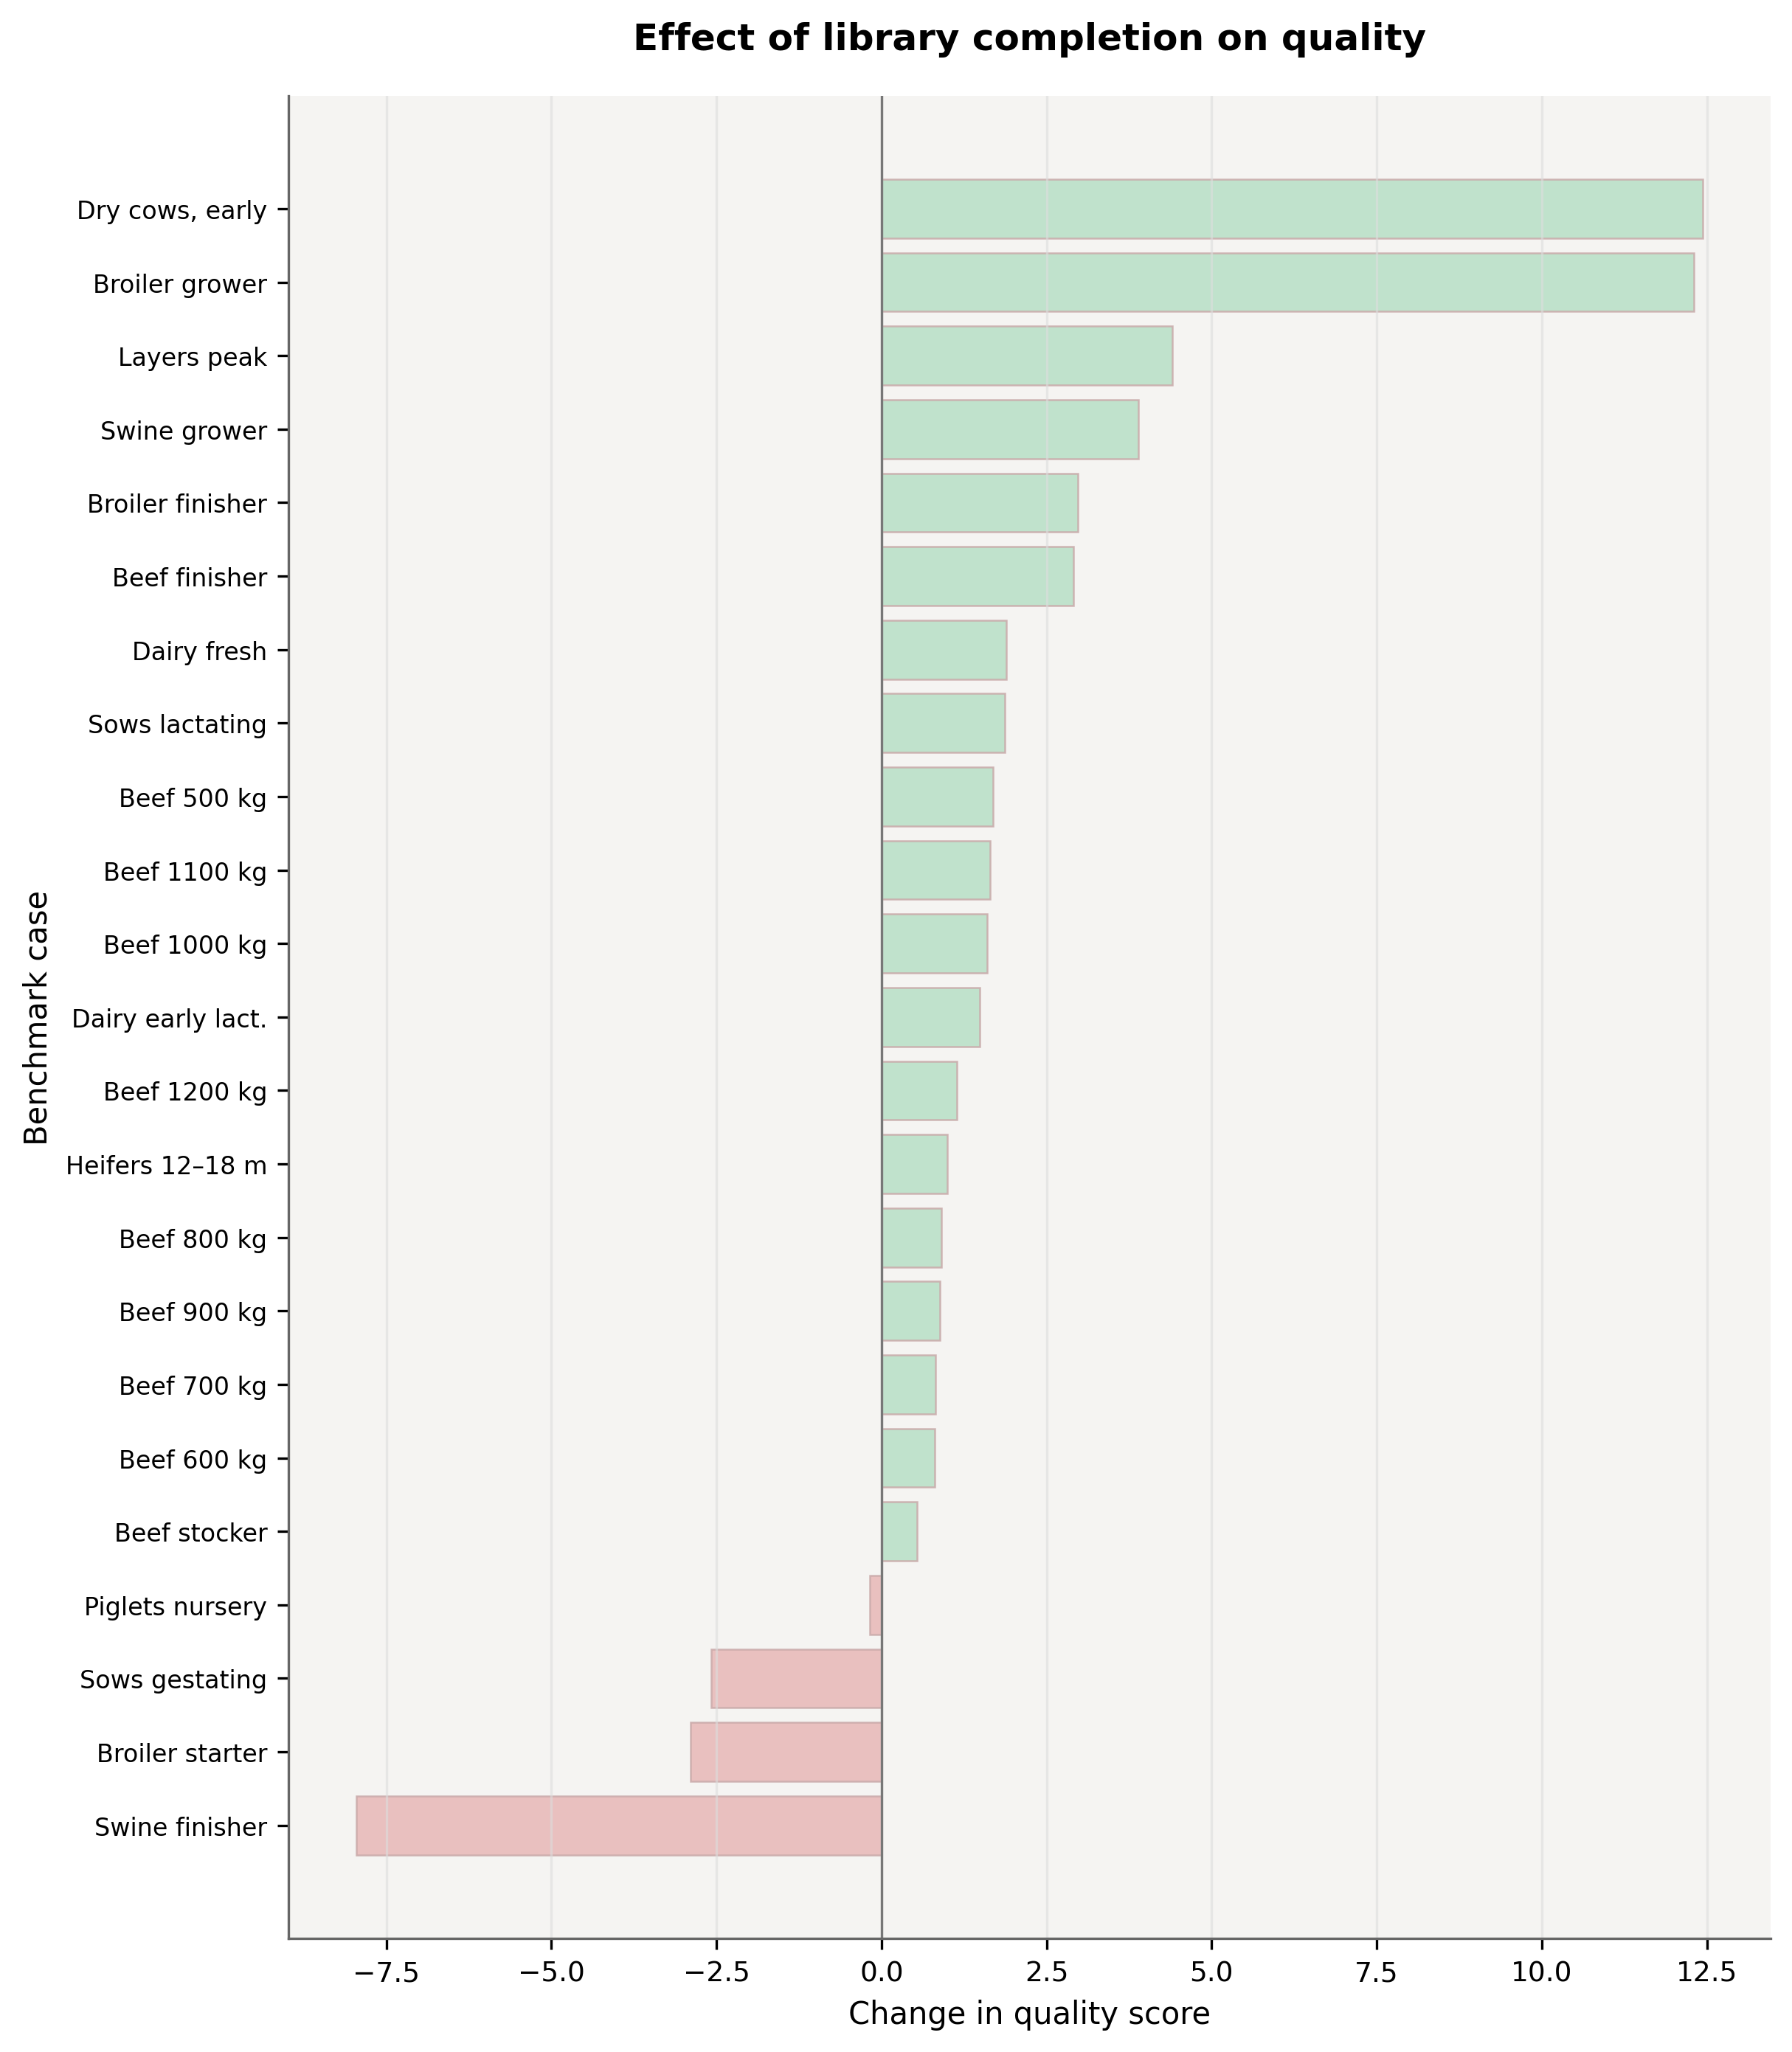
\includegraphics[width=0.85\textwidth]{Figure_3_Quality_Delta.png}
    \caption{Quality Delta (difference in coverage indices) resulting from transitioning from automated construction to balancing a user-defined ration skeleton.}
    \label{fig:qualitydelta}
\end{figure}

An in-depth analysis of systematic deficiencies was conducted for monogastric animals (swine and poultry; Supplementary Tables S5, S6). The heatmap (Figure \ref{fig:heatmap-en}) illustrates the cumulative severity of deviations. The primary limiting factors remained phosphorus, calcium density, vitamin D3, sodium, lysine or lysine-proxy constraints, and the sum of methionine and cystine depending on species and stage.

\begin{figure}[htbp]
    \centering
    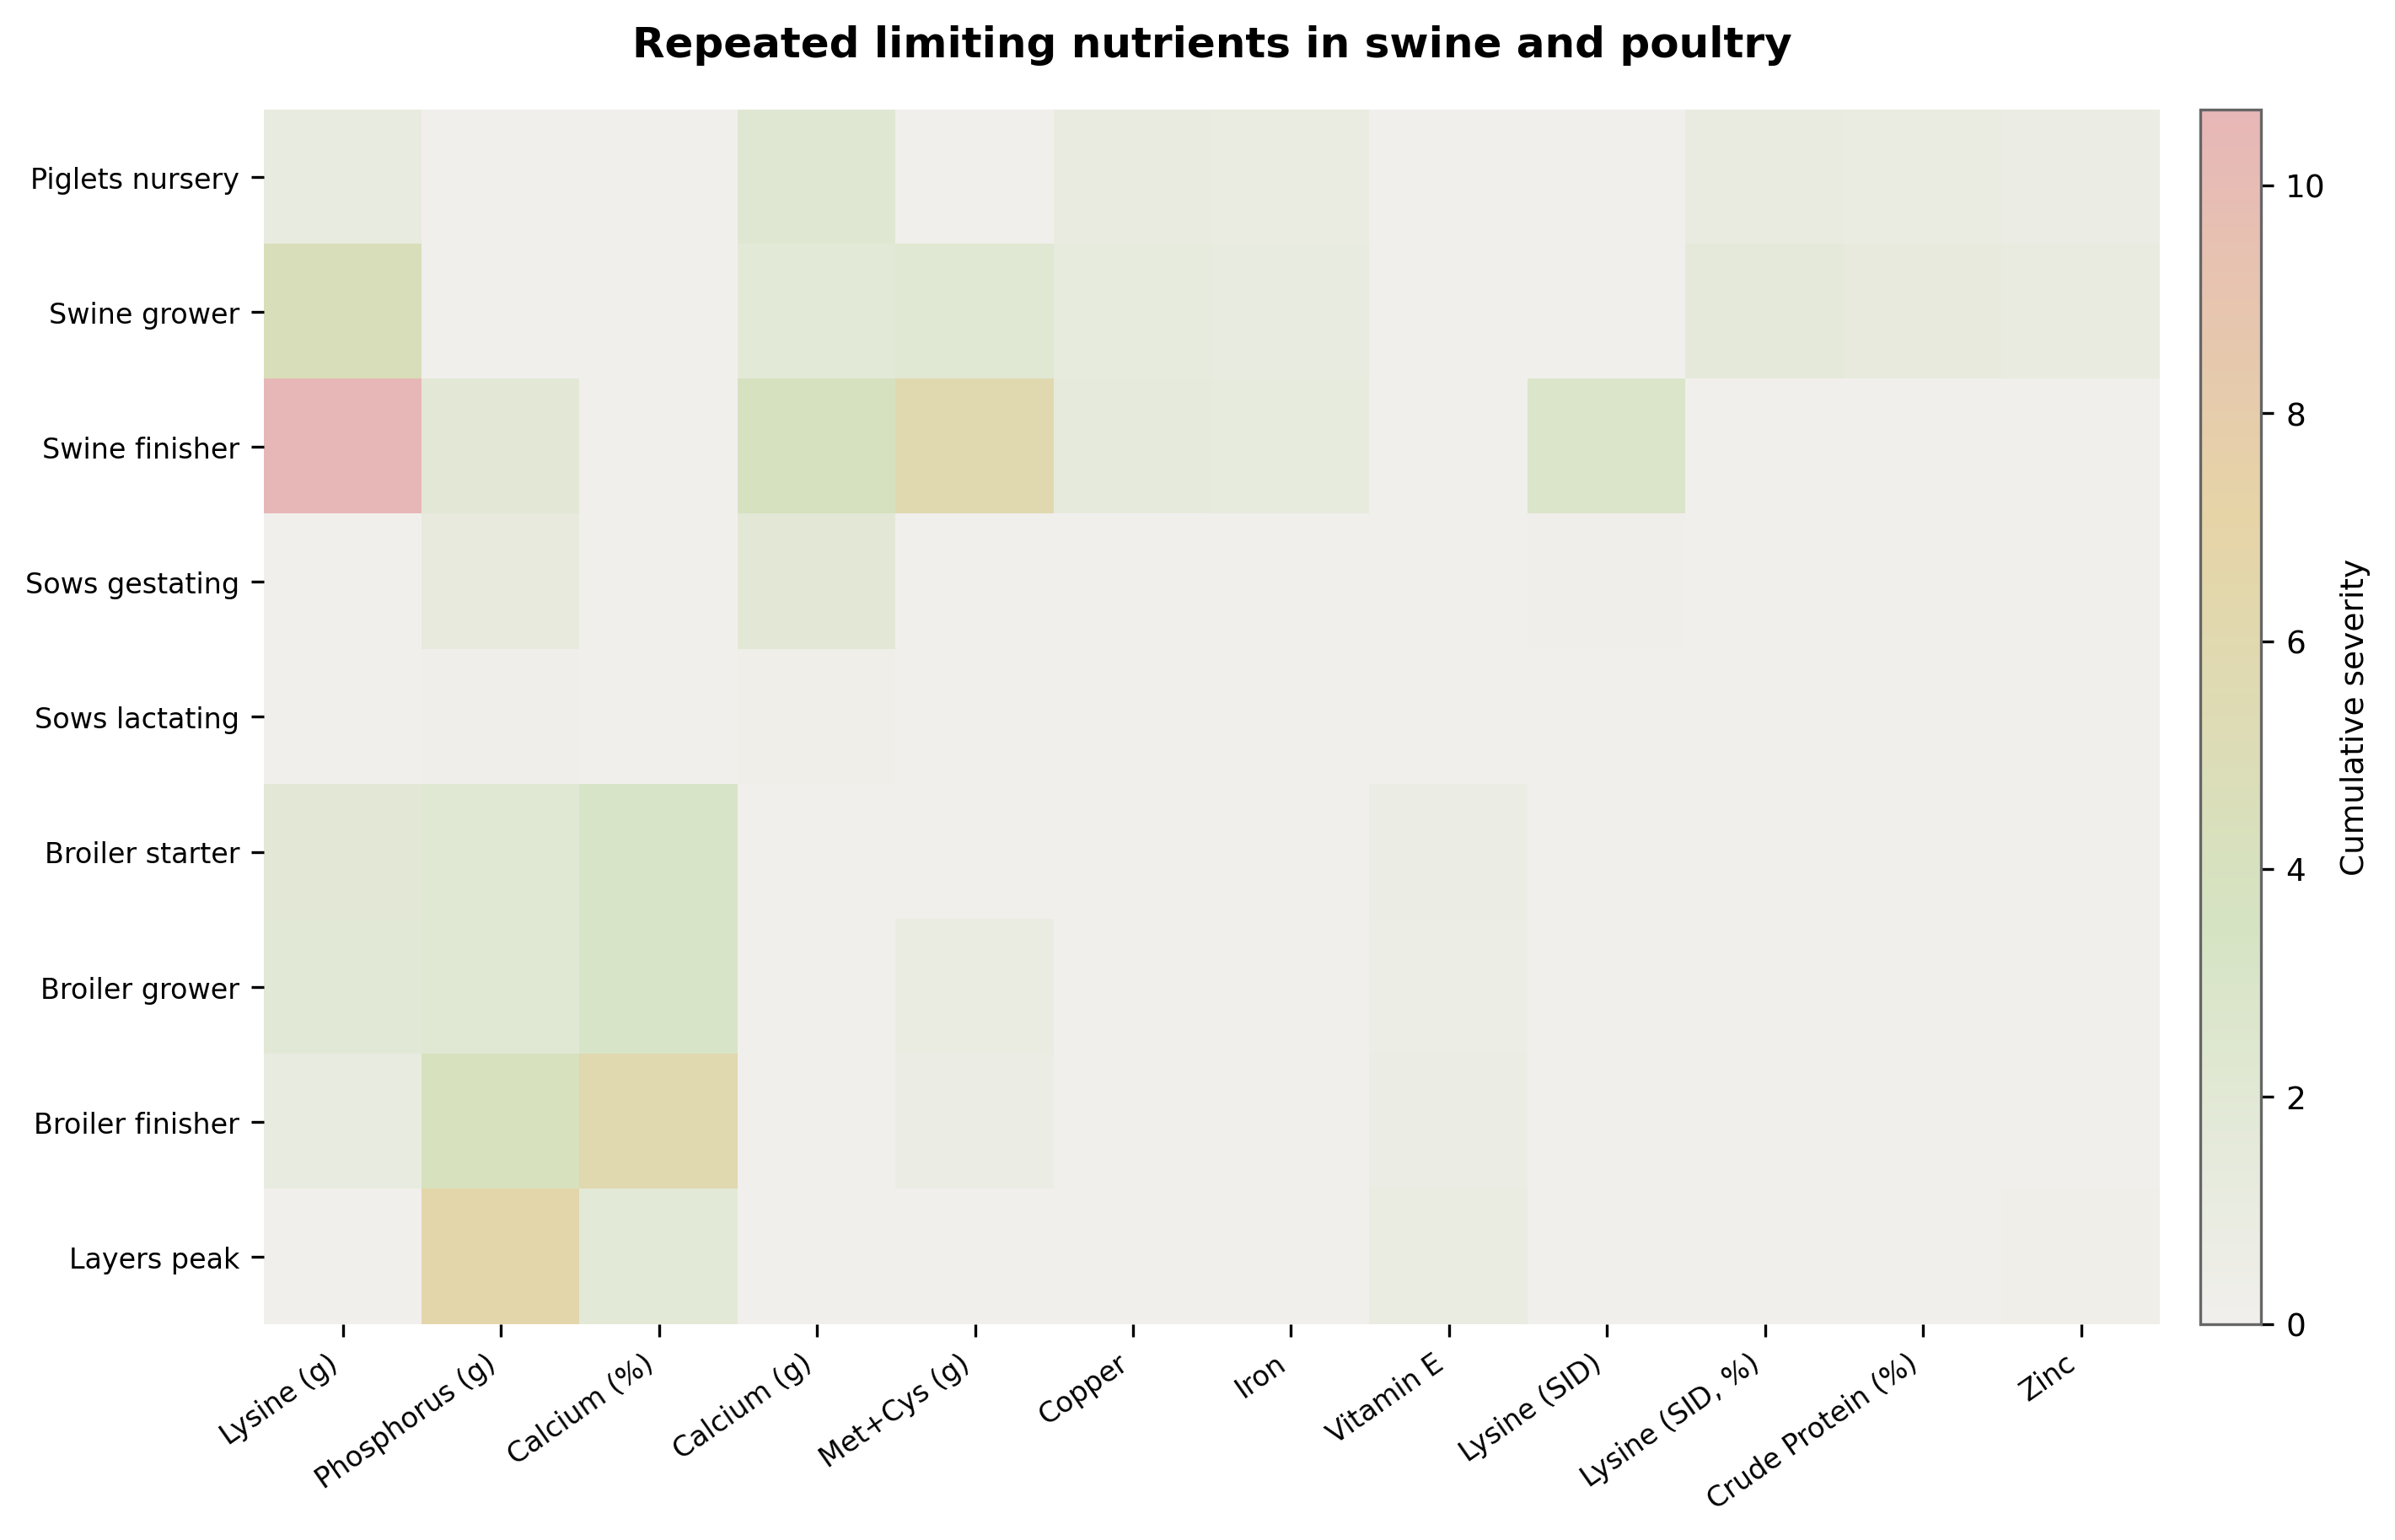
\includegraphics[width=0.92\textwidth]{Figure_5_Heatmap.png}
    \caption{Cumulative severity of nutrient deficiencies (by magnitude of deviation from the norm) in completed rations for swine and poultry scenarios.}
    \label{fig:heatmap-en}
\end{figure}

\subsection{Economic analysis and LLM evaluation}\label{subsec:economic}

The average cost of a ration was 183.0 RUB/day. Figure \ref{fig:costscatter} demonstrates a non-linear relationship between cost and workflow, forming species-specific clusters. For cattle, two rations with the same number of ingredients could differ markedly in cost and utility depending on the balance of roughages and concentrates. In poultry, relatively small additions of nutritionally dense feeds could substantially improve norm coverage.

\begin{figure}[htbp]
    \centering
    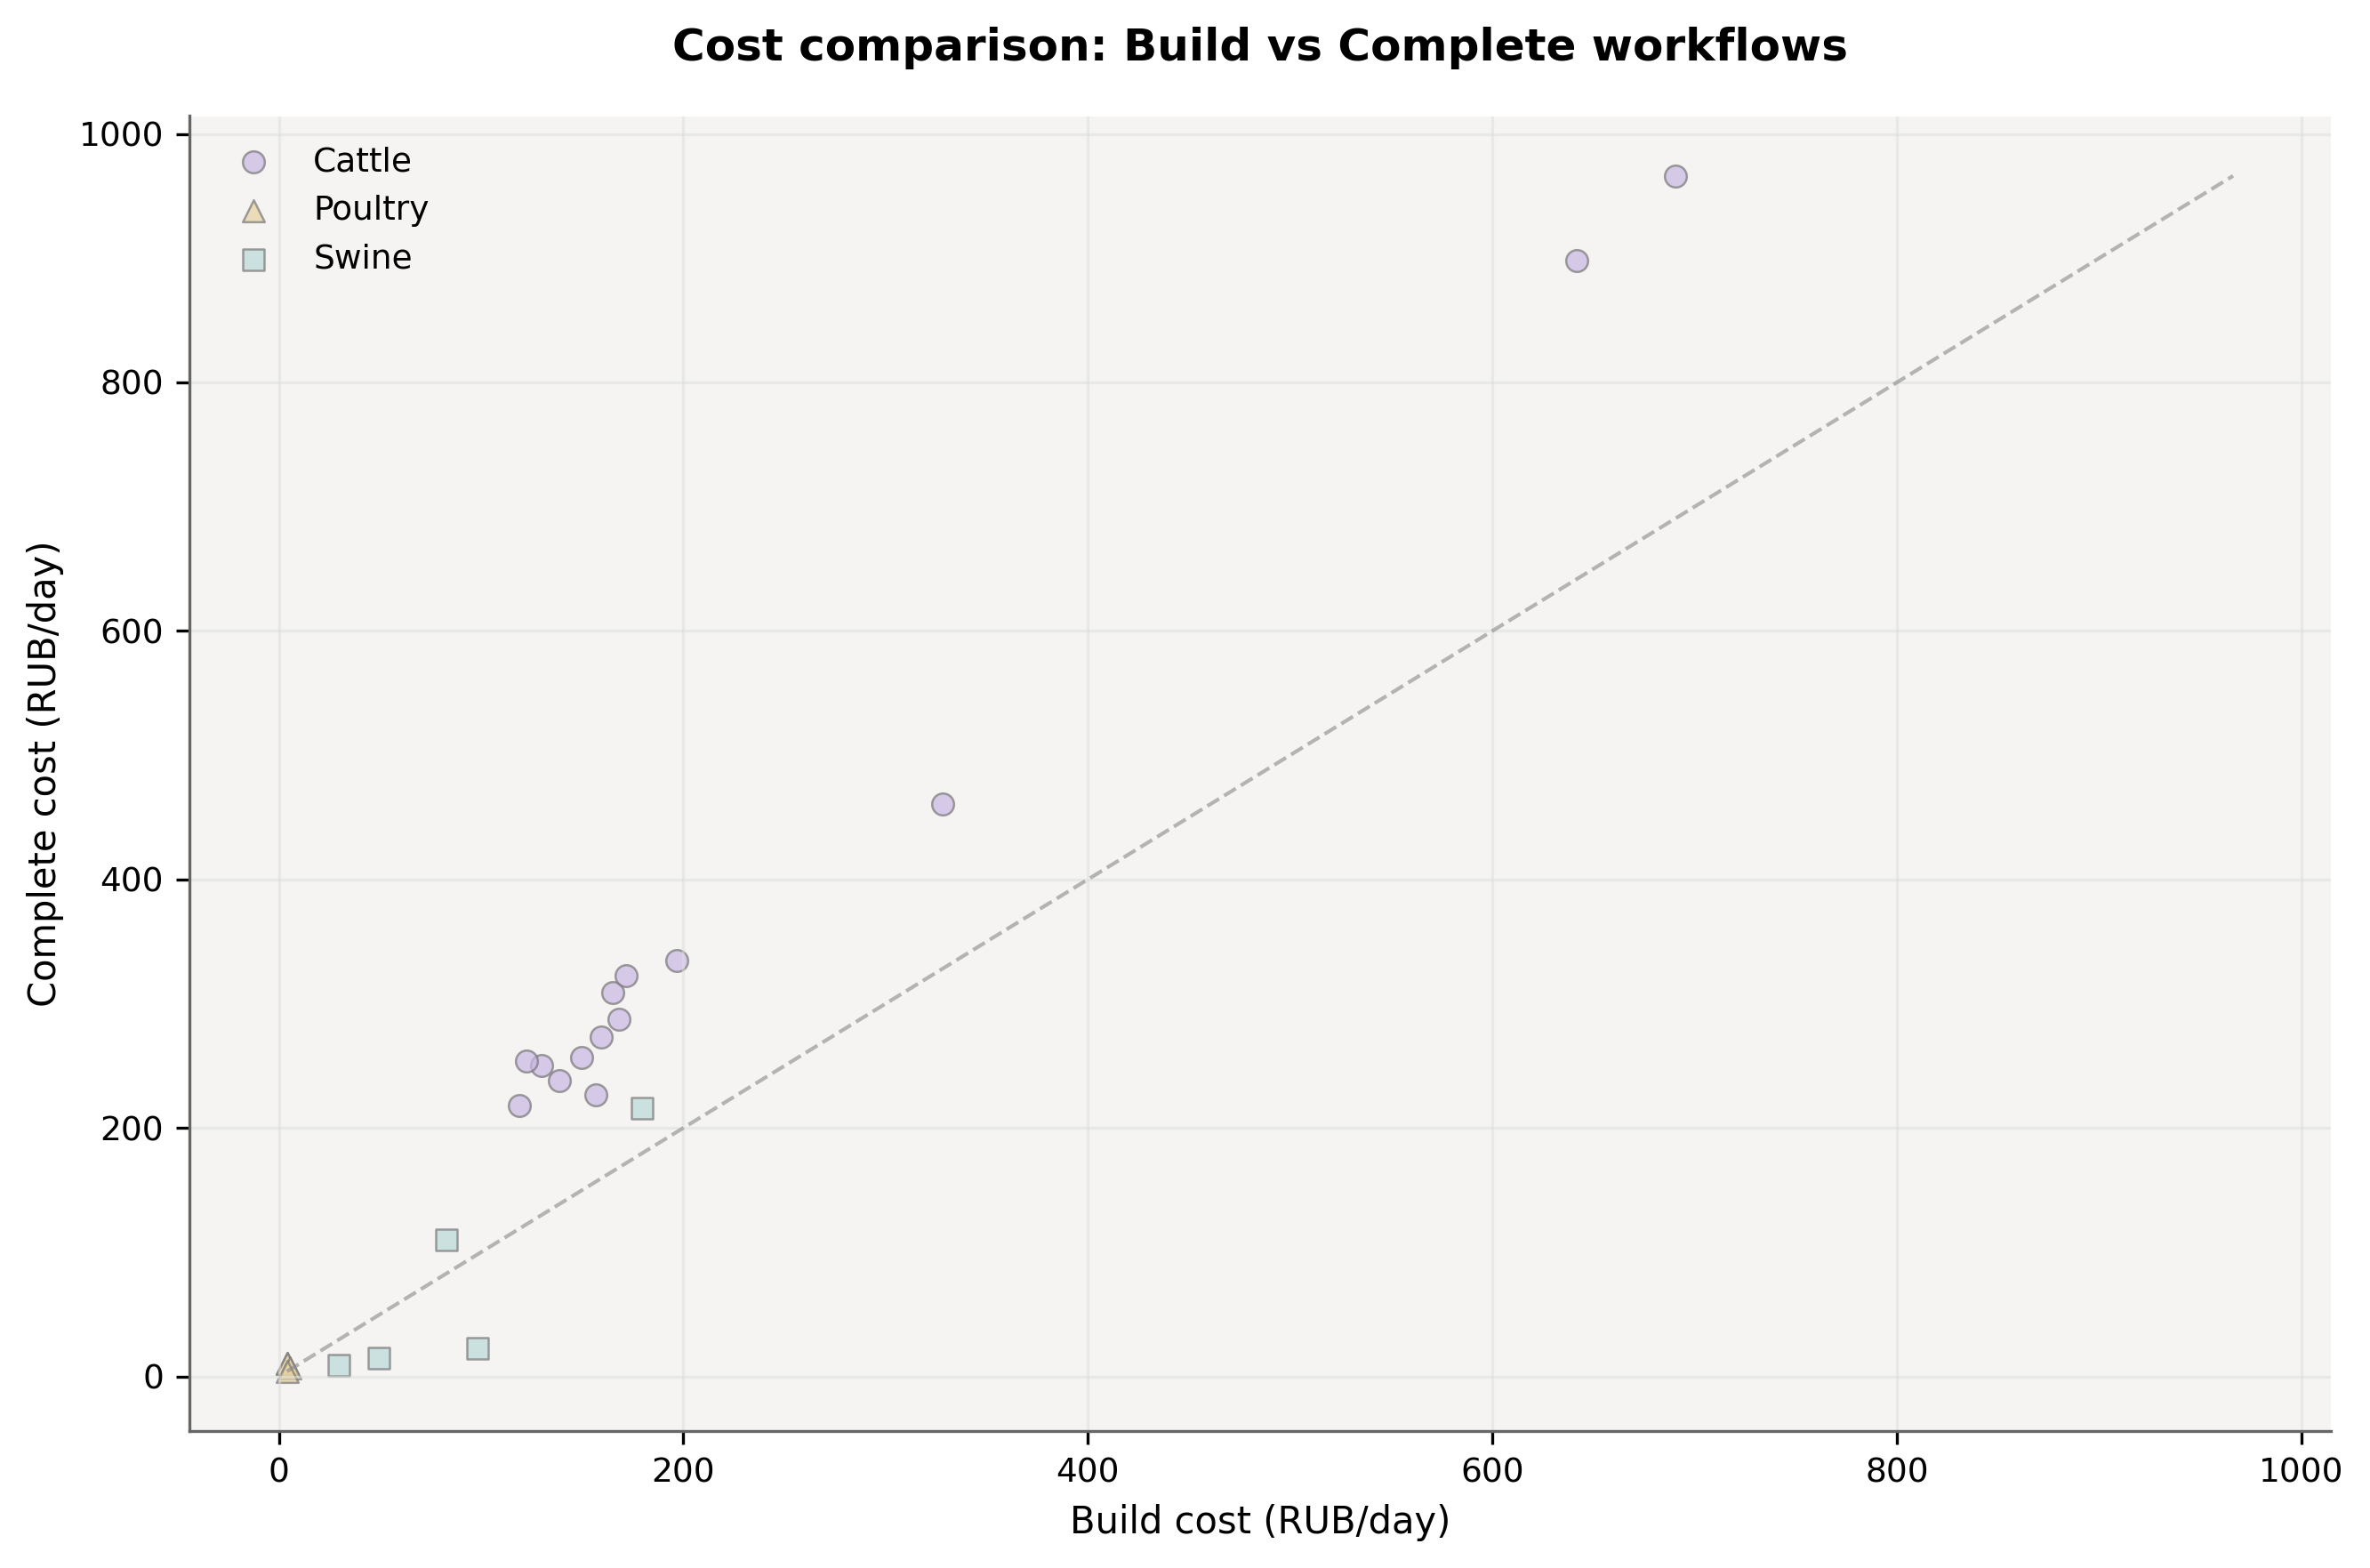
\includegraphics[width=0.82\textwidth]{Figure_6_Cost_Scatter.png}
    \caption{Dependence of ration cost on the applied optimization mode, with clustering by animal species.}
    \label{fig:costscatter}
\end{figure}

Evaluation of the local consultant agent across both tested Qwen configurations (Table \ref{tab:llm-eval}) showed limited usefulness. Neither configuration improved the aggregate benchmark over the other: both the 4B/4096 and 9B/2048 settings produced limiting-nutrient recall@3 of 0.17, grounded recommendation rate@3 of 0.67, lookup accuracy of 0.50, and overall applicability of 34.2/100. Importantly, the added benchmark telemetry showed that these results were obtained without hidden model or context fallback. The present limitation is therefore not a silent infrastructure downgrade but inadequate task performance within the bounded consultant role.

\begin{table}[width=\linewidth,cols=6,pos=htbp]
\caption{Bounded in-application consultation benchmark of local Qwen 3.5 configurations across 12 tasks.}\label{tab:llm-eval}
\begin{tabular*}{\tblwidth}{@{}LLLLLL@{}}
\toprule
Configuration & Limiting recall@3 & Grounded rate@3 & Lookup accuracy & Overall applicability & Interpretation \\
\midrule
Qwen 3.5 4B @ 4096 & 0.17 & 0.67 & 0.50 & 34.2/100 & Inadequate for dependable consultation \\
Qwen 3.5 9B @ 2048 & 0.17 & 0.67 & 0.50 & 34.2/100 & No aggregate gain under constrained context \\
\bottomrule
\end{tabular*}
\end{table}

\section{Discussion}\label{sec:discussion}

The benchmark confirms that the three Felex workflows should be interpreted as different practical operating modes rather than as equivalent solver settings. \texttt{selected\_only} is extremely fast but structurally limited by the user-provided feed set. \texttt{build\_from\_library} offers the broadest search, but even this mode remained sub-second on average in the current benchmark. \texttt{complete\_from\_library} provided the best balance in the current benchmark, combining materially better norm coverage with runtime short enough for routine specialist use. For an applied livestock audience, this is the most relevant result: Felex performs best when it extends an expert-defined ration skeleton rather than when it is asked to replace expert input entirely.

This positioning also fits the current software field. Felex is not a replacement for enterprise formulation suites or integrated farm-management platforms \citep{datacor2026, korall2026, onecow2026}. Its more defensible niche is a local, transparent instrument for specialists who need explicit workflows, mixed normative support, and reduced dependence on proprietary cloud stacks. That niche is particularly relevant in Russian operating conditions, where localized tools exist \citep{deltakorm2026, winmix2026} but open, benchmarked, locally deployable options remain limited.

The nutritional behavior of the current engine is consistent with practical formulation logic. For cattle, metabolizable-energy accounting remains a pragmatic compromise for a cross-species tool \citep{inra2018, volden2011, kalashnikov2003}. For monogastric animals, the recurrent pressure around digestibility-aware amino-acid constraints and phosphorus supports the continued importance of digestibility-aware formulation \citep{stein2007, nRC2012, pomar2021, deLange2012, vanmilgen2015}. The observed hard-constraint pass rate near 65\% should therefore not be read as simple algorithmic failure; it also reflects imperfect feed data, sparse price anchors, and the biological difficulty of satisfying all tiers simultaneously from a constrained library. The benchmarked nutrient contour, matrix definitions, and category-level feed-base composition used to interpret these patterns are documented in Supplementary Tables S7, S8, and S9, respectively. The hierarchical LP strategy and fallback soft-goal step remain reasonable for practical ration construction under those conditions \citep{rehman1987}.

The local agent results require a more cautious interpretation than the previous manuscript draft suggested. Under a bounded in-application consultation benchmark, both tested Qwen configurations reached the same low aggregate adequacy score, and the larger 9B model did not improve on the 4B model when constrained to a smaller context window. Because benchmark telemetry showed no hidden model or context fallback, these weak results are attributable to task performance rather than to silent infrastructure degradation. At the current stage, the agent is best understood as an experimental explanatory layer that can sometimes summarize, contextualize, and propose candidate adjustments while leaving responsibility for interpretation with the specialist.

Several limitations follow directly from the repository state and benchmark evidence. First, the optimization core remains linear, whereas nonlinear, multi-objective, stochastic, and evolutionary approaches may better represent some biological trade-offs and composition uncertainty \citep{li2022nonlinear, uyeh2018, uyeh2019, das2023, agrawal2025, kumar2025}. Second, the regional feed database should be expanded and continuously curated; the present benchmark-ready catalog is useful, but it still rests on a modest number of direct price anchors. Third, the norm engine should be extended with richer factorial derivatives, especially for regional practice, stage-specific production states, and uncertainty-aware sensitivity analysis. Fourth, the local agent layer should not be expanded by model scaling alone: under the present bounded benchmark, a larger model at a smaller context window did not improve adequacy. Future work should therefore combine improved regional feed data, richer norm derivation, uncertainty analysis, explainable recommendation traces, and, for the agent layer, better task grounding and domain adaptation rather than simple parameter growth.

\section{Conclusion}\label{sec:conclusion}

Felex demonstrates that a locally deployable livestock ration platform can combine transparent optimization workflows, mixed normative support, and a practical desktop runtime without relying on a cloud-first architecture. In its current state, the strongest use case is supportive ration building for specialists in small farms and animal businesses, especially where regional adaptation and operational autonomy matter. The present benchmark supports that practical positioning, while also showing clear limits in database coverage, uncertainty handling, and the adequacy of the local agent for dependable consultation. Those limits define the next development agenda more clearly than any claim of automation maturity.

% Author contributions (CRediT taxonomy) - printed via \printcredits before references

% Conflict of Interest
\section*{Declaration of Competing Interest}

The authors declare that they have no known competing financial interests or personal relationships that could have appeared to influence the work reported in this paper.

% Funding
\section*{Funding}

This research received no external funding.

% Data Availability
\section*{Data Availability Statement}

The Felex source code is available at \url{https://github.com/danilkotelnikov/Felex}. The canonical optimization benchmark artifact used in this manuscript is stored at \url{https://github.com/danilkotelnikov/Felex/tree/main/.claude/benchmarks}, with the primary JSON at \url{https://github.com/danilkotelnikov/Felex/blob/main/.claude/benchmarks/results/benchmark_results.json}. The bounded local-agent benchmark artifacts used in this revision are stored at \url{https://github.com/danilkotelnikov/Felex/tree/main/deliverables/agent_publication_benchmark_2026-04-03_qwen4b_4096} and \url{https://github.com/danilkotelnikov/Felex/tree/main/deliverables/agent_publication_benchmark_2026-04-03_qwen9b_2048}. The raw normalized feed export is available at \url{https://github.com/danilkotelnikov/Felex/blob/main/database/output/feeds_database.json}. Additional data and scripts are available from the corresponding author upon reasonable request.

% Acknowledgments
\section*{Acknowledgments}

The authors thank the developers of the \texttt{good\_lp} library, the Ollama ecosystem, and the maintainers of open agricultural standards and reference resources that made this work possible.

% AI Use Declaration
\section*{Declaration of generative AI and AI-assisted technologies in the manuscript preparation process}

During the preparation of this work the authors used \textbf{Anthropic Claude} (Claude Opus 4.6 and Claude Sonnet variants, \url{https://www.anthropic.com/claude}) and \textbf{OpenAI Codex} (\url{https://openai.com/index/openai-codex/}) in order to assist with literature synthesis, code documentation review, manuscript language editing, LaTeX formatting, and benchmark-audit documentation. After using these tools, the authors reviewed and edited the content as needed and take full responsibility for the content of the published article.

% Print CRediT authorship contributions
\printcredits

% Bibliography
\bibliographystyle{cas-model2-names}
\bibliography{felex_references}

\end{document}
